\documentclass[../diagrams.tex]{subfiles}

\begin{document}
\label{diagrams:class_diagrams}

\subsubsection{Model systemu}

Aby nadzorca wiedział jak zarządzać systemem potrzebuje przechowywać model systemu.
Poniższa struktura danych przedstawia aktualny stan całego systemu.

\begin{figure}[!h]
	
	\centering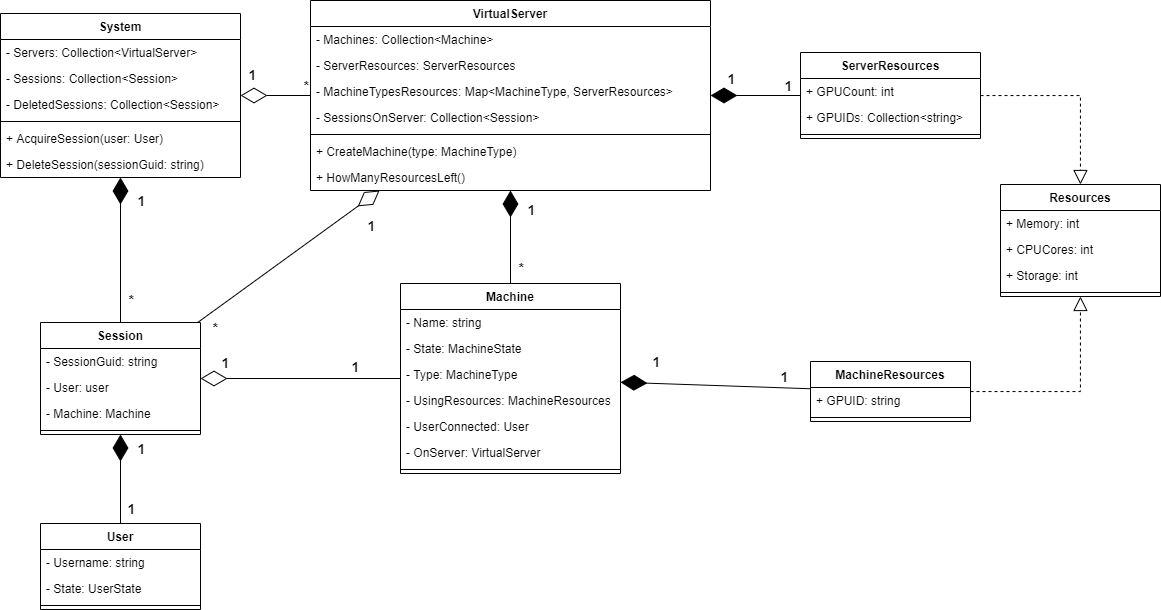
\includegraphics[width=\textwidth]{class_diagrams/system_model.png}
	
	\vskip-1.5ex
	
	\caption{Diagram klas dla modelu systemu}
	\label{figure:diagrams:class_diagrams:system_model}
\end{figure}

W skład tego modelu wchodzą informacje o:
\begin{enumerate}
	\item Dostępnych serwerach wirtualizacji.
	\item Dostępnych zasobach na serwerach.
	\item Aktualnie działających maszynach, ich typach oraz zajmowanych przez nie zasobach.
	\item Aktualnie trwających sesjach z użytkownikami.
\end{enumerate}

\end{document}